\usepackage{amsmath,amssymb,amsthm}

\usepackage{fullpage}
\usepackage{hyperref}
\usepackage{color}
\usepackage[barr]{xy}
\usepackage{todonotes}
\usepackage{tikz}
\usepackage{tikz-qtree}
\usepackage{stmaryrd}
\usepackage{mathpartir}
\usepackage{layout}
\usepackage[margin=1.1in]{geometry}

%% \usepackage{nobibprint}

\newtheorem{thm}{Theorem}
\newtheorem{lemma}[thm]{Lemma}
\newtheorem{corollary}[thm]{Corollary}
\newtheorem{definition}[thm]{Definition}
\newtheorem{remark}[thm]{Remark}
\newtheorem{proposition}[thm]{Proposition}
\newtheorem{notn}[thm]{Notation}
\newtheorem{observation}[thm]{Observation}

\newcommand{\cat}[1]{\mathbb{#1}}
\newcommand{\catobj}[1]{\mathsf{Obj}(\cat{#1})}
\newcommand{\catop}[1]{\mathbb{#1}^{\mathsf{op}}}
\newcommand{\sets}[0]{\mathsf{Sets}}
\newcommand{\homs}[2]{\mathsf{Hom}[#1,#2]}
\newcommand{\cur}[0]{\mathsf{cur}}
\newcommand{\curi}[0]{\mathsf{cur}^{-1}}
\newcommand{\app}[0]{\mathsf{app}}
\newcommand{\id}[0]{\mathsf{id}}
\newcommand{\injl}[0]{\mathsf{inj_l}}
\newcommand{\injr}[0]{\mathsf{inj_r}}
\newcommand{\pow}[1]{\mathcal{P}(#1)}
\newcommand{\cpy}[0]{\textcopyright}
\newcommand{\lett}[3]{\mathsf{let}\,#1 = #2\,\mathsf{in}\,#3}

% Commands that are useful for writing about type theory and programming language design.
\newcommand{\case}[4]{\text{case}\ #1\ \text{of}\ #2\text{.}#3\text{,}#2\text{.}#4}
\newcommand{\interp}[1]{[\negthinspace[#1]\negthinspace]}
\newcommand{\normto}[0]{\rightsquigarrow^{!}}
\newcommand{\join}[0]{\downarrow}
\newcommand{\redto}[0]{\rightsquigarrow}
\newcommand{\nat}[0]{\mathbb{N}}
\newcommand{\terms}[0]{\mathcal{T}}
\newcommand{\fun}[2]{\lambda #1.#2}
\newcommand{\CRI}[0]{\text{CR-Norm}}
\newcommand{\CRII}[0]{\text{CR-Pres}}
\newcommand{\CRIII}[0]{\text{CR-Prog}}
\newcommand{\subexp}[0]{\sqsubseteq}
\newcommand{\napprox}[2]{\lfloor #1 \rfloor_{#2}}
\newcommand{\interpset}{\mathcal{I}}
\newcommand{\powerset}[1]{\mathcal{P}(#1)}
\newcommand{\vinterp}[1]{\mathcal{V}[\negthinspace[#1]\negthinspace]}
\newcommand{\vbinterp}[2]{\bar{\mathcal{V}}_{#1}[\negthinspace[#2]\negthinspace]}
\newcommand{\ginterp}[1]{\mathcal{G}[\negthinspace[#1]\negthinspace]}
\newcommand{\dinterp}[1]{\mathcal{D}[\negthinspace[#1]\negthinspace]}
\newcommand{\tinterp}[1]{\mathcal{T}[\negthinspace[#1]\negthinspace]}


\title{\vspace{-50px}CRII: SHF: A New Foundation for Attack Trees Based on Monoidal Categories}
\author{Harley Eades III, Computer and Information Sciences, \\Augusta University}
\date{\vspace{-22px}}
\begin{document}
\maketitle  

\begin{full}
%% \layout
\section{Overview}
\label{sec:overview}

\textbf{Attack trees} are a modeling tool, originally proposed by
Bruce Schneier \cite{Schneier:1999}, which are used to assess the
threat potential of a security critical system.  Attack trees have
since been used to analyze the threat potential of many types of
security critical systems, for example, cybersecurity of power grids
\cite{Ten:2007}, wireless networks \cite{Reinhardt:2012}, and many
others.  Attack trees consists of several goals, usually specified in
English prose, for example, ``compromise safe'' or ``obtain
administrative privileges'', where the root is the ultimate goal of
the attack and each node coming off of the root is a refinement of the
main goal into a subgoal.  Then each subgoal can be further refined.
The leaves of an attack tree make up the set of base attacks.  Subgoals
can be either disjunctively or conjunctively combined.

%% Extensions Of ATREES:
%%   - Attack nets
%%   - Sequential conjunction
\textbf{Extensions of attack trees.}  There have been a number of
extensions of attack trees to include new operators on goals.  One
such extension recasts attack trees into attack nets which have all of
the benefits of attack trees with the additional benefit of being able
to include the flaw hypothesis model for penetration testing
\cite{McDermott:2001}.  A second extension adds sequential conjunction
of attacks, that is, suppose $A_1$ and $A_2$ are attacks, then
$A_1;A_2$ is the attack obtained by performing $A_1$, and then
executing attack $A_2$ directly after $A_1$ completes
\cite{Jhawar:2015}.

\textbf{The need for a foundation.}  Attack trees for real-world
security scenarios can grow to be quite complex.  The attack tree
presented in \cite{Ten:2007} to access the security of power grids has
twenty-nine nodes with sixty counter measures attached to the nodes
throughout the tree.  The details of the tree spans several pages of
appendix.  The attack tree developed for the border gateway protocol
has over a hundred nodes \cite{Convey:2003}, and the details of the
tree spans ten pages.  Manipulating such large trees without a formal
semantics can be dangerous.

%% Semantics of ATREES:
%%   - Boolean logic
%%   - Attack nets (2000)
%%   - Multisets (2006)
%%   - Series-parallel graphs (extension of multisets) (2015)
\textbf{The formal semantics of attack trees.} The leading question
the field is seeking to answer by giving a mathematical foundation to
attack trees is ``what is an attack tree?''  There have been numerous
attempts at answering this question.  For example, attack trees have
been based on propositional logic and De Morgan Algebras
\cite{Kordy:2014,Kordy:2012,Pietre-Cambacedes:2010}, multisets
\cite{Mauw:2006}, Petri nets \cite{McDermott:2001}, tree automata
\cite{Camtepe:2007}, and series parallel graphs
\cite{Jhawar:2015}. \textbf{There is currently no known semantics of
  attack trees based in category theory}.

By far the most intuitive foundation of attack trees is propositional
logic or De Morgan algebras, however, neither of these properly
distinguish between attack trees with repeated subgoals.  If we
consider each subgoal as a \textbf{resource} then the attack tree
using a particular resource twice is different than an attack tree
where it is used only once.  The multiset semantics of attack trees
was developed precisely to provide a resource conscious foundation
\cite{Mauw:2006}. The same can be said for the Petri nets semantics
\cite{McDermott:2001}.  A second benefit of a semantics based in
multisets, Petri nets, and even tree automata is that operators on
goals in attack trees are associated with concurrency operators from
process algebra.  That is, the goals of an attack tree should be
thought of as being run concurrently -- it seems this connection to
process algebra has been overlooked.  Furthermore, when moving to
these alternate foundations \textbf{the intuitiveness and elegance of
  the propositional logic semantics is lost}.  Lastly, existing work
has focused on specifically what an attack tree is, and has not sought
to understand what the theory of attack trees is.

\textbf{Category Theory.}  Each of the various existing mathematical
foundations attempt to answer the question ``what is an attack
tree?'', but they are all seemingly very different mathematical
structures.  Is there a unifying core foundation common to all of
these existing foundations? A categorical foundation will answer this
question in the positive. The powers of category theory -- an abstract
branch of mathematics first proposed by Samuel Eilenberg and Saunders
Mac Lane \cite{MacLane:1971} -- are its ability to abstract away
unneeded details from a mathematical structure, and its ability to
form relationships between seemingly unrelated mathematical
structures.  For example, intuitionistic logic and the
$\lambda$-calculus both correspond to cartesian closed categories, and
hence, are different perspectives of the same theory
\cite{Lambek:1980}.  A categorical foundation of attack trees will
result in the most basic mathematical foundation of attack trees,
furthermore, it will reveal a relationship between all of the existing
mathematical foundations, and lastly, it will reconnect attack trees
with logic, but also forge new connections with functional programming
languages and formal verification through the Curry-Howard-Lambek
correspondence.  This implies that by giving attack trees a semantics
in category theory one obtains a more powerful semantic analysis and
the ability to \textbf{derive a programming language that can not only
  define attack trees, but also reason about them using formal
  verification} (Section~\ref{sec:prop-lina}).  In addition, the
various graphical languages used in category theory,
\cite{Selinger:2009}, may lead to new graphical tools for threat
analysis.

\textbf{This Proposal.} I propose to found attack trees in linear
logic rather than propositional logic by giving attack trees a
semantics in symmetric monoidal categories.  A semantics in symmetric
monoidal categories is a generalization over the previous forms of
models of attack trees.  Multisets and Petri nets are examples of
symmetric monoidal categories \cite{Brown:1991,Tzouvaras:1998}.
Furthermore, symmetric monoidal categories are a categorical model of
linear logic \cite{dePaiva:2014}, thus regaining the elegant
connection between attack trees and logical formulas.  The connection
to linear logic also opens the door to a connection between threat
analysis using attack trees and process algebra such as Petri nets,
but also Chu spaces \cite{Pratt:1999}, dialectica spaces
\cite{dePaiva:2006b}, and session types
\cite{Wadler:2012,Caires:2010}.  I and my trainees will fully develop
the semantics of attack trees in symmetric monoidal categories and
show that not only can attack trees be modeled by these types of
categories, but so can a range of their extensions like attack trees
with sequential conjunction.  We will also investigate new attack tree
operators based on the connection to process algebra.  Then we will
develop a new formal system called Lina for \underline{Lin}ear Threat
\underline{A}nalysis (Section~\ref{sec:prop-lina}).  Lina will be a
statically typed linear polymorphic functional domain-specific
programming language designed to construct, manipulate, and prove
properties of attack trees.  Lina will represent attack trees as
linear types, and thus, programs between these types will be
considered transformations of attack trees.  The semantics of Lina
will also be in symmetric monoidal categories forming a tight
correspondence with the semantics of attack trees.  This system will
be the first threat analysis tool to support proving properties of
attack trees, thus \textbf{connecting software verification to threat
  analysis.}  Finally, new threat analysis tools can be built on top
of Lina.

\textbf{Outcomes and impact.}  By basing attack trees in linear logic
this work will connect threat analysis to resource conscious logics,
software verification and process algebra.  This will open the door
for many interesting future projects in all of these areas of study.
This work will also provide new extensions of attack trees and new
extensions of linear logic, both of which will have a significant
impact on the field.  Lina's representation of attack trees as types
and transformations as programs is a completely novel representation
of attack trees.  Furthermore, Lina has practical significance due to
its ability to not only define and manipulate attack trees, but
actually prove properties about attack trees.

\textbf{PI qualifications.} I have extensive experience designing and
analyzing both simply typed and dependently typed programming
languages and logics.  As part of my dissertation I was a member of
the Trellys project
\cite{Casinghino:2012,Kimmel:2013,Sjoberg:2015,Sjoberg:2012} in which
I contributed to the design of a dependently typed functional
programming language called Separation of Proof from Program
($\text{Sep}^3$) whose design is now detailed in my dissertation
\cite{Eades:2014b,Kimmel:2013}.  The second major part of my
dissertation was dedicated to the meta-theoretic analysis of various
type theories.  First, I studied a new proof technique for proving
normalization of simply typed and predicative polymorphic type
theories called hereditary substitution, and then proved completeness
of a new logic and simple type theory called dualized simple type
theory \cite{Eades:2014b}.
% section overview (end)

\end{full}
\begin{full} 
\section{Linear Attack Trees in Symmetric Monoidal Categories}
\label{sec:attack_trees_in_monoidal_categories}
In this section we give some preliminary work on giving attack trees a
semantics in symmetric monoidal categories.  This semantics is the
starting point for the Lina programming language
implementation. Suppose we wanted to assess the threat of whether an
attacker could steal the social security number of person
$\mathsf{X}$. An attack tree could be used and might look something
like the following:
\begin{center}
  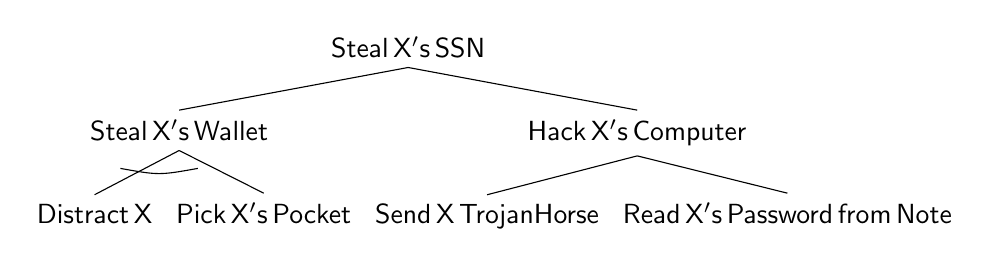
\begin{tikzpicture}
\Tree [.{$\mathsf{Steal\,X's\,SSN}$}
          [.{$\mathsf{Steal\,X's\,Wallet}$} {$\mathsf{Distract\,X}$}
            [.{$\mathsf{Pick\,X's\,Pocket}$} ] ]
          [.{$\mathsf{Hack\,X's\,Computer}$} {$\mathsf{Send\,X\,Trojan Horse}$}
            [.{$\mathsf{Read\,X's\,Password\,from\,Note}$} ] ] ]
\draw (-104pt,-40pt) .. controls (-90pt, -42.5pt) .. (-76pt,-40pt);
\end{tikzpicture}
\end{center}
The root of the attack tree is the goal of the attack, and then this
goal is refined into two new subgoals which are to either steal
$\mathsf{X}$'s wallet or to hack their computer.  Then these two goals
can be refined further.  Note that there is an arc between the two
edges connecting the subgoals of the goal to steal $\mathsf{X}$'s
wallet.  This arc signifies that the two subgoals must be done
together.  These are often called conjunctive subgoals while all of
the other goals are disjunctive.  The graphical presentation of attack
trees is very appealing, but for large complex systems it becomes hard
to utilize.  So attack trees are often presented in the form of a
script. A third representation of attack trees uses $n$-ary operators;
for example, we can represent the tree from above by the following:
\[
\begin{array}{rll}
  \mathsf{Steal\,X's\,SSN} & = & (\mathsf{Steal\,X's\,Wallet}) + (\mathsf{Hack\,X's\,Computer})\\
  \mathsf{Steal\,X's\,Wallet} & = & (\mathsf{Distract\,X}) \otimes (\mathsf{Pick\,X's\,Pocket})\\
  \mathsf{Hack\,X's\,Computer} & = & (\mathsf{Send\,X\,Trojan Horse}) + (\mathsf{Read\,X's\,Password\,from\,Note})\\
\end{array}
\]

After developing an attack tree it is common to add a weight to each
node of the tree.  This weight can be thought of as the cost of
conducting that attack.  Then attacks with high cost can be considered
as unlikely and safely ignored.  For example, we can give weights to
the attack tree given above:
\begin{center}
  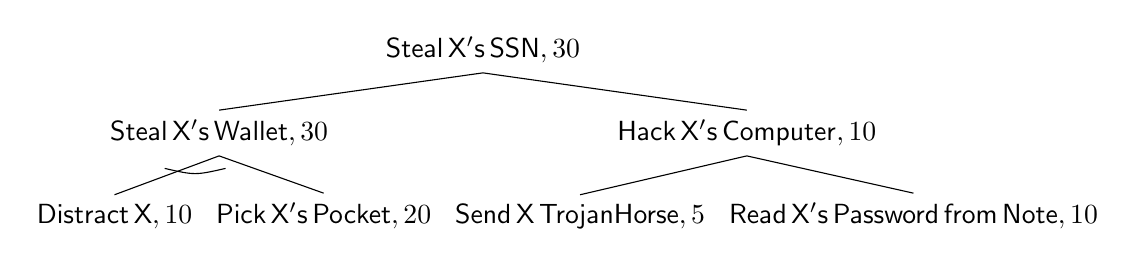
\begin{tikzpicture}
\Tree [.{$\mathsf{Steal\,X's\,SSN},30$}
          [.{$\mathsf{Steal\,X's\,Wallet},30$} {$\mathsf{Distract\,X},10$}
            [.{$\mathsf{Pick\,X's\,Pocket},20$} ] ]
          [.{$\mathsf{Hack\,X's\,Computer},10$} {$\mathsf{Send\,X\,Trojan Horse},5$}
            [.{$\mathsf{Read\,X's\,Password\,from\,Note},10$} ] ] ]
\draw (-115pt,-40pt) .. controls (-104pt, -42.5pt) .. (-93pt,-40pt);
\end{tikzpicture}
\end{center}
After giving attacks costs different projections can be conducted on
the attack tree to project out attacks meeting some criteria.
We concentrate on attack trees without weights or any additional
structures on the nodes here.

At this point we give the formal definition of a new form of attack
tree we call linear attack trees (or just attack trees).
\begin{definition}
  \label{def:unlabeled-attack-trees}
  \textbf{Linear Attack trees} are defined by the following grammar:
  \[
  \begin{array}{lll}
    B & ::= & b_1 \mid \cdots \mid b_n\\
    A & ::= & B \mid \otimes(A,\ldots,A) \mid \times(A,\ldots,A) \mid +(A,\ldots,A) \mid \cpy(A)\\
  \end{array}
  \]
  We call $B$ the set of base attacks, and we will often treat the
  attack tree operators as infix operators.  The following rules
  define the attack tree reduction relation:
  \begin{center}
    \vspace{-25px}
    \begin{mathpar}
      \inferrule* [right=assoc] {
        \,
      }{(A \otimes B) \otimes C \redto A \otimes (B \otimes C)}
      \and
      \inferrule* [right=dist] {
        \,
      }{A \otimes (B + C) \redto (A \otimes B) + (A \otimes C)}
    \end{mathpar}
  \end{center}
  The previous rules can be applied on any well-formed subattack
  tree. The equivalence relation, denoted $\equiv$, on attack trees is
  defined as the reflexive, symmetric, and transitive closure of the
  reduction relation $\redto$.
\end{definition}
The two rules we consider here, association and distribution, are
similar rules considered by Mauw and Oostdijk \cite{Mauw:2006}. One of
the novel aspects of this work is we treat each attack as a process
and the attack tree operators as concurrency operators on processes.
Now suppose $A_1$ and $A_2$ are two attack trees.  Then the attack
tree defined by $A_1 \otimes A_2$ is the process where attack $A_1$ is
run parallel to attack $A_2$, this is called parallel composition of
attack trees. The attack tree $A_1 \times A_2$ corresponds to the
process that executes attacks $A_1$ and $A_2$ in any order.  The
attack tree that executes attacks $A_1$ or $A_2$ in any order is
defined by $A_1 + A_2$.  This interpretation suggests that attacks are
resources and as such cannot be freely duplicated or deleted, and
thus, we add an explicit operator, $\cpy(A)$, which should be read as
``$A$ can be copied.''  Our semantics will enforce that the only
attack trees that can be copied must be under the copy operator.

Our goal of this section is to give a semantics of attack trees, as
defined above, in symmetric monoidal categories\footnote{Suppose $f :
  A \to B$ and $g : B \to C$ are two arbitrary morphisms of some
  category $\cat{C}$, then we denote their composition by $f;g : A \to
  C$.} with some additional structure.
\begin{definition}
  \label{def:monoidal-category}
  A \textbf{symmetric monoidal category}, $(\cat{C}, I, \otimes)$, is
  a category with a binary endofunctor $\otimes : \cat{C} \times
  \cat{C} \to \cat{C}$, an object $I \in \catobj{C}$, natural
  isomorphisms $\lambda_A : I \otimes A \to A$, $\rho_A : A \otimes I
  \to A$, and $\alpha_{A,B,C} : A \otimes (B \otimes C) \to (A \otimes
  B) \otimes C$, and a natural transformation $\beta_{A,B} : A \otimes
  B \to B \otimes A$.  The natural isomorphisms and transformations
  are subject to several coherence equations that we omit; see
  \cite{MacLane:1971}.
\end{definition}
Basic symmetric monoidal categories are enough to model attack trees
which solely consist of the parallel composition operator $\otimes$,
and thus, to model the other operators we must extend monoidal
categories with some additional structure.
\begin{definition}
  \label{def:additive-linear-categories}
  An \textbf{additive linear category}, $(\cat{C}, I, \otimes, 1,0,
  \times, +)$ is a symmetric distributive monoidal category,
  $(\cat{C}, I, \otimes)$, with products and coproducts.  Being
  distributive means that for any objects $A,B,C \in \catobj{C}$,
  there is a natural isomorphism, $\mathsf{d}_{A,B,C} : A \otimes (B +
  C) \to (A \otimes B) + (A \otimes C)$.
\end{definition}
At this point additive linear categories contain enough structure to
model all of attack trees, but the copy operator.
\begin{definition}
  \label{def:affine-categories}
  A \textbf{linear attack model} consists of the following data:
  \begin{itemize}
  \item An additive linear category, $(\cat{L}, I, \otimes, 1,0,\times,
  +)$,
  \item a distributive category\footnote{A cartesian category with
    coproducts where products distribute over coproducts}, $(\cat{C},
    1,0,\times, +)$,
  \item a pair of symmetric monoidal functors $F : \cat{C} \to
    \cat{L}$ and $G : \cat{L} \to \cat{C}$, such that, $F$ and $G$
    form a symmetric monoidal adjunction\footnote{For the definitions
      of symmetric monoidal functor/adjunction see
      \cite{Benton:1994}.}.
  \end{itemize}
\end{definition}

The previous definition is based on the notion of a linear/non-linear
model of intuitionistic linear logic \cite{Benton:1994}.  Intuitively,
think of the category $\cat{L}$ as the model of resource conscious
attack trees, and the category $\cat{C}$ as the model of attack trees
based on propositional logic \cite{Kordy:2014,Kordy:2012}.  Then the
adjoint functors $F$ and $G$ are translations between the two types of
models.  These do not create an isomorphism, but only a relationship.

An analogy might help with understanding how to view the adjunction.
Suppose there is an Earth like planet called planet $X$.  Now planet
$X$ is just like Earth, but it has a slightly less powerful force of
gravity.  This implies that all of Earth's physics can be translated
to the physics of planet $X$ by weakening gravity, and planet $X$'s
physics can be translated to Earth's physics by strengthening gravity.
Thus, we have an adjunction between planet $X$'s physics and Earth's
physics.

We will see that the composition of $F$ and $G$ will model the copy
operator.  The beautiful part of this model over existing models is
that it can handle attack trees based on resources, attack trees based
propositional logic, and a hybrid of both.  The copy operator gives us
the best of both worlds.
\begin{definition}
  \label{def:attack-tree-interpretation}
  Suppose $B$ is a set of basic attacks, and $(\cat{L}, \cat{C}, G,
  F)$ is a linear attack model, $\mathsf{ob} : B \to \catobj{L}$ is an
  injective function, and $\mathsf{op} \in \{\otimes,\times,+\}$.
  Then we define the interpretation of attack trees as objects of
  $\cat{L}$ by induction as follows:
  \begin{center}
    \begin{math}
      \begin{array}{lll}
        \interp{b} & = & \mathsf{ob}(b)\\
        \interp{A_1 \mathrel{\mathsf{op}} A_2} & = & \interp{A_1} \mathrel{\mathsf{op}} \interp{A_2}\\
        \interp{\cpy A} & = & F(G(\interp{A}))\\
      \end{array}
    \end{math}
  \end{center}
  We will now denote $G;F$ by $\cpy$.  The interpretation of the
  reduction relation for attack trees as morphisms of $\cat{L}$ is as
  follows:
  \begin{center}
    \begin{math}
      \begin{array}{lll}
        \interp{(A \otimes B) \otimes C \redto A \otimes (B \otimes C)} & = & \alpha^{-1}_{\interp{A},\interp{B},\interp{C}}\\
        \interp{A \otimes (B + C) \redto (A \otimes B) + (A \otimes C)} & = & \mathsf{d}_{\interp{A},\interp{B},\interp{C}}\\
      \end{array}
    \end{math}
  \end{center}
\end{definition}
There are two main points that one should take away from the previous
definition.  The first is that the attack trees are simply objects of
the category, but even more so, the morphisms are semantically valid
transformations on the attack trees.  Finally, the second point is
that the copy operator can be seen as a gateway traveling from linear
logic (monoidal category) to propositional logic (cartesian category).
This then implies that proofs of equivalences of two attack trees
corresponds to proofs of isomorphisms between morphisms of the model.
In fact, it is straightforward to prove the following.

\begin{lemma}[Soundness]
  \label{lemma:soundness}
  For any attack trees $A$ and $B$, if $A \equiv B$, then $\interp{A}
  = \interp{B}$.
\end{lemma}

Linear attack models as defined above are left abstract, but our
interpretation shows that any concrete mathematical structure that can
be proven to be an attack model is sufficient to use to reason about
attack trees.  For example, Petri nets have been used to model attack
trees \cite{McDermott:2001}, but Petri nets can be modeled by
dialectica categories \cite{Brown:1991} which themselves have been
shown to be an example of a linear/non-linear model of linear logic,
and thus, essentially corresponds to a linear attack model
\cite{Eades:2015}.
% section attack_trees_in_monoidal_categories (end)
\section{Proposed: The Lina Implementation}
\label{sec:prop-lina}
My trainees and I will develop an implementation of a system for
specifying and reasoning about attack trees called Lina for Linear
Threat Analysis.  Lina will consist of a core language and a surface
language.  The core language will include a decidable type checker
using term annotations on types; note that type checking becomes
undecidable in the presence of parametric polymorphism
\cite{Wells:1999}.  Programming with annotations can be very
cumbersome, and so the surface language will use local type inference
\cite{Pierce:2000} to alleviate some of the burden from annotations.
However, the surface language will provide further conveniences in the
form of automation, to be used with labeled attack trees, and
graphical representations of attack trees based on the various
graphical languages used in category theory \cite{Selinger:2009}.

\subsection{The Lina Core Language}
\label{subsec:core_language}

The core language of Lina will have the tightest correspondence with
the attack model semantics of attack trees.  It will be an extension
of Benton's linear/non-linear term assignment \cite{Benton:1994}.  The
extensions will include second-order polymorphism, linear additive
products and linear additive coproducts.  The addition of second-order
polymorphism raises the issue of extending our attack model to ensure
that the correspondence with Lina is upheld.  We conjecture that this
will be possible by extending our attack model to a hyperdoctrine
model in a similar way to Seely's hyperdoctrine model for classical
linear logic \cite{Seely:1990}.  A last extension from Benton's term
assignment is that we will add type annotations to terms to make type
checking decidable.

\textbf{Labeled attack trees.}  So far the core language has mainly
been concerned with the shape of attack trees, and whether or not one
attack tree is the same as another attack tree with a different shape.
We will add the ability to label attack trees with weights and do
projections on attack trees.  There is one hurdle that needs to be
addressed and that is whether or not Lina should allow reasoning
between attack trees with labels.  This extension might result in
having to extend the equivalence relation on attack trees to account
for labels.  I conjecture that by layering a semi-ring over the attack
model we could extend the core language with abstract labels to
facilitate this addition.  This would be similar to how Maw and
Oostdijk \cite{Mauw:2006} handle labels in their model.

\textbf{Verification.} The Lina core language can be seen as
essentially being derived from the attack model using the
Curry-Howard-Lambek correspondence.  Objects will correspond to types,
and morphisms will correspond to well-typed programs.  Thus, defining
an attack tree will correspond to defining a type.  Then performing
semantically valid transformations on attack trees, say from attack
tree $A_1$ to attack tree $A_2$, corresponds to defining a program
whose input type is $A_1$ and whose output type is $A_2$.  This
program can be seen as evidence that $A_2$ is semantically related to
$A_1$, and thus, can be seen as a proof that $A_1$ implies $A_2$.  In
fact, we could prove that $A_1$ and $A_2$ are equivalent if we can
write programs from $A_1$ to $A_2$ and vice versa.  This type of
verification is called interactive theorem proving and it is the locus
of proof in interactive theorem provers such as Coq
\cite{CoqRefMan:2008} and Agda \cite{Norell:2009}.

Combing this with polymorphism allows for the construction of generic
attack tree transformations.  In this way we can view type variables
as holes that can be filled with attack trees.  Thus, providing a
mechanism for defining new attack tree operators within Lina without
necessarily having to extend the core language.
% subsection core_languages (end)

\subsection{The Lina Surface Language}
\label{subsec:surface_language}

The Lina surface language will provide a more user-friendly
programming environment by alleviating the burden of programming with
type annotations using local type inference, and by providing a means
of writing mutually recursive functions much like one would find in
Haskell and Agda.  Attack trees are types, and these types can become
quite large, so to facilitate their construction the surface language
will also provide type-level recursive global definitions.

\textbf{A graphical language.} We will also develop a web based
graphical interface for proving equivalences of attack trees.  For
example, suppose we wanted to prove that the attack tree $A \otimes (B
\otimes C)$ is equivalent to $(A \otimes B) \otimes C$.  Then instead
of providing the proof explicitly using the programming constructs one
can provide a proof using an alternative graphical calculus that then
translates to the traditional surface language.  The graphical
language will support the definition of an attack tree by placing
nodes and edges on a canvas, but in addition it will provide the user
with several predefined graphical gadgets that describe equations
between the shapes of two subtrees.  In the core language these
gadgets are represented by isomorphisms between types that represent
the subtrees.  The user can use these graphical equations to conduct
semantically valid transformations on attack trees in a completely
graphical fashion.  I conjecture this to be possible by exploiting the
work of Blute et al. \cite{Blute:1996a} and/or the work on open graphs
used by the Quantomatic application \cite{Dixon:2011,Dixon:2010}.
% subsection surface_language (end)

\section{Personnel, Equipment, and Work Plan}
\label{sec:personnel_and_work_plan}
\textbf{Personnel.} I am requesting funds to support six
undergraduates and two Ph.D. students.  The Ph.D. students will be
hired during the summers of the first and second years.  During the
first year, the Ph.D. student will aid me in extending the linear
attack tree semantics to include more attack tree operators, and the
student during the second year will aid me in conducting the
meta-theoretic analysis of Lina.

The undergraduate employees during the first year will aid me in
developing the Lina core language.  Then in the second year the
undergraduate students will aid me in developing the surface language.
More precisely, the undergraduate students during the second year will
develop the graphical interface to the surface language.

Augusta University does not at this time have a graduate program in
computer science, and thus, the Ph.D. students recruited to work with
me will come from another university.  During the summer of 2015
Augusta University established the Cyber Institute.  It is the goal of
the institute as well as the computer and information sciences
department to eventually add a graduate program in computer science.
Visiting Ph.D. students will contribute to this eventual goal.  This
would also be a valuable experience for the Ph.D. students, because
they would get the chance to work with a researcher outside of their
university.  The Ph.D. students will need a basic foundation in either
category theory or the meta-theoretic analysis of functional
programming languages.  To recruit these students I plan to advertise
the opportunity to US based universities.

I plan to recruit the undergraduates who will aid me in the
implementation of the Lina core and surface languages from my
upper-level programming languages course.  In this course I teach the
basics of the design and implementation of functional programming
languages using Haskell.  So these students will already have the
necessary introduction to Haskell, the language we will be developing
Lina in, and the implementation of programming languages needed for
the project.

The undergraduates that will aid me in implementing the graphical
interface to the Lina surface language will not need to know Haskell
or how to implement functional programming languages, but will need a
foundation in web development.  I plan to recruit these students from
the pool of students who have taken the web development course that is
taught in my department.

\ \\
\noindent
\textbf{Equipment.}  To develop and host the Lina graphical web
application I am asking for the funds to buy and host a development
server.  It will be hosted and maintained by the GRU Cyber Institute
at Augusta University.

%% \ \\
%% \noindent
%% \textbf{Workshop.} I am also requesting funds to host a two day
%% workshop for graduate students called ``Category Theory and its
%% Applications in Computer Science.''  I plan to invite approximately
%% fifteen graduate students and two invited speakers.  The two days will
%% primarily consist of talks from graduate students from other
%% universities doing work in computer science using category theory.
%% This would be both a wonderful opportunity for graduate students to
%% get a chance to present their work and obtain feedback, and provide a
%% time for the undergraduates at Georgia Regents University to network
%% with graduate students and spark interest for continuing on to
%% graduate school.
% section personnel_and_work_plan (end)

\section{Broader Impacts of the Proposed Work}
\label{sec:broader_impacts_of_the_proposed_work}

The primary impact of this work is in the advancement of the state of
the art in the mathematical foundations of threat analysis and the
tool support for threat analysis.  The additional impact is in
mentoring and teaching.

\subsection{Advances over Previous Work}
\label{subsec:advances_over_previous_work}
The mathematical foundations of attack trees proposed here is the
first foundation based in category theory and linear logic.  Past
mathematical foundations are either very complex, or do not treat
goals as resources.  In
Section~\ref{sec:attack_trees_in_monoidal_categories} we give the
first mathematical foundation of attack trees that provides both a
semantics for a resource conscience interpretation simultaneously with
an interpretation in propositional logic. It is possible to have the
best of both worlds!  By founding attack trees in category theory we
are able to derive a core programming language
(Section~\ref{subsec:core_language}) with the ability to define and
reason about attack trees.  Then by creating a surface language over
the core we will have the first threat analysis tool that is
semantically correct, and with the ability to not only define and
manipulate attack trees, but verify properties about them formally.
Lastly, this work is the first to apply formal verification to threat
analysis.
% subsection advances_over_previous_work (end)

\subsection{Teaching and Mentoring}
\label{subsec:teaching_and_mentoring}

\textbf{Teaching.} I plan to create a section on domain specific
programming languages in my upper-level undergraduate programming
languages course where my students will explore the design of Lina and
conduct some case studies using Lina.

\ \\
\noindent
\textbf{Undergraduate Research.}  I am the first person in my family
to go to college, and I was well within my twenties when I entered my
bachelor's program making me a non-traditional student.  This is not
an uncommon story of the vast majority of the students at Augusta
University.  Most are U.S. native non-traditional or even
post-baccalaureate students.  Due to the close proximity to Fort
Gordon a large percentage of our students are either active military
or military veterans.

I am dedicated to working with non-traditional students -- 30\% of
undergraduate students enrolled at Augusta University are
non-traditional students (25 years of age or older) -- military
veterans -- 9\% of undergraduate students at Augusta
University are either military verterns, active military, or are
members of a military family -- and people of minority groups -- 32\%
of undergraduate students at Augusta University are people of
minority groups -- by providing them with rich research
experiences. Undergraduate research opportunities at my university
have been sparse, and so this proposal will contribute to creating
more research possibilities for these types of students.  %% The workshop
%% proposed in Section~\ref{sec:personnel_and_work_plan} will also give
%% all the students of the Computer and Information Sciences department
%% the opportunity to attend a research workshop and allow them to
%% interact with graduate students.  This workshop would be the first
%% computer science workshop to be held at Georgia Regents University.

Undergraduate students working on a research project like the one
being proposed here should get a chance to do more than the expected
tasks, for example, just writing programs.  I want to include the
students in all aspects of the project including the design and
theoretical aspects of the project.  This will give them a chance to
really experience research.  Furthermore, I want them to get the
experience of writing up the research, and so they will be included in
the final stages of the project as well.  This experience could help
convince the types of students listed above to pursue a career in
research and go to graduate school when they would otherwise never
think that such a career path was possible for them.

\ \\
\noindent
\textbf{Graduate Research.} At this time Augusta University
does not have a graduate program in computer science.  However, the
Computer and Information Sciences department does have plans of adding
one in the future.  The visiting Ph.D. students will aid in helping
these plans move forward by sparking interest in our department at
other schools, but by also giving the department an opportunity to
work with the visiting graduate students.

In addition, the visiting graduate students will help spark
undergraduate interest in attending graduate school. Both types of
students will have a chance to work together, where otherwise the
students at Augusta University would not have such a chance to
gain a first hand perspective of graduate school and research.
Lastly, the visiting graduate students will have a chance to
experience helping mentoring undergraduate students in a research
project.
% subsection teaching_and_mentoring (end)
% section broader_impacts_of_the_proposed_work (end)

\section{Prior NSF Support}
\label{sec:prior_nsf_support}
During graduate school I was a contributing member of the NSF funded
Trellys project which was a collaboration between Aaron Stump and his
students at the University of Iowa, Stephanie Weirich and her students
at the University of Pennsylvania, and Tim Sheard and his students at
Portland State University to design a new general purpose
dependently-typed functional programming language that supports
type-based verification.  The primary aim of the project was
understanding how to mix type-based verification with general
recursion.

My primary contribution to this project was to the design and analysis
of the core language. The design space for the core language is quite
large and as a team we made the decision to investigate three
different language designs, one by each school. At the University of
Iowa we designed a language called Separation of Proof and Program
(Sep3)
\cite{Kimmel:2013,Kimmel:2012,Eades:2014b}. It is well known that if
one designs their richly typed functional programming language such
that every program defined within it terminates, then one can consider
the programs as proofs and their types predicates. Thus, verification
of programs turns into writing other programs viewed as
proofs. However, with respect to Trellys, this design no longer
applies, because we want to have general recursion; hence, not every
program terminates. Sep3 overcomes this by separating the two
worlds. Then, we link the two fragments together, so that the logical
fragment can verify properties of the programs written inside the
programmatic fragment.

The second part of my contribution to the Trellys project was to the
meta-theoretic analysis of the logical fragment of the Trellys core
language.  My advisor and I investigated the potential of using a
technique known as hereditary substitution -- due to Watkins et
al. \cite{Watkins:2004} -- to prove weak normalization of the logical
fragment.  Hereditary substitution is a function that substitutes the
arguments of functions for parameters, but if a new function call is
created it hereditarily reduces it. Now it turns out that to show the
logical fragment is terminating it suffices to show the hereditary
substitution function is terminating. This technique is simpler than
other known techniques, and is easier to formalize in a proof
assistant. We were the first to apply hereditary substitution to show
weak normalization of predicative-polymorphic programs, and we were
the first to extend this technique to programming languages with
control operators \cite{Eades:2010,Eades:2013,Eades:2014b}.

The project was very collaboration based and I got the chance to
collaborate across schools.  Annually for the lifetime of the project
all of the contributors of the project would gather at one of the
three universities.  During these annual meetings we would present all
of our recent results, and work closely on problems we have
encountered and work together to get past those problems.  I had the
pleasure to visit and work with Tim Sheard and his students at
Portland State University.  Lastly, I spent the summer of 2013 working
closely with Stephanie Weirich and her students in which we worked on
extending dependent types to classical type theories and control
operators.  In addition, during my visit I presented my thesis work on
hereditary substitution to the Penn PL club.  These collaborations
were hugely important for my education and research, and I want to
give similar experiences to my current and future students.  This
proposal has the potential to begin offering such experiences.
% section prior_nsf_support (end)


\end{full}
%% \nocite{*}
\bibliographystyle{plain}
\bibliography{refs}



